\section{Algebraic MultiGrid (AMG) Preconditioners}~\label{AMG}
%

MultiGrid methods are widely used as preconditioners of iterative
Krylov solver for sparse linear systems. 
They are very efficient methods, having linear computational
complexity and hence perfect scalability, when 
sparse and large linear systems stemming
from the discretization of some scalar elliptic Partial Differential
Equations (PDEs) have to be solved~\cite{Vassilevski2008}. 
Many efforts are related to extend their efficient applicability also
to more general systems, in particular in the direction of a complete
algebraic approach, where no information on a possible geometric
origin of the problem is exploited. In this last case, they are named
Algebraic MultiGrid (AMG) or Algebraic Multilevel
methods~\cite{Stuben2001}. 
MultiGrid methods rely their efficiency on the recursive application
of two complementary processes: {relaxation and coarse-grid
  correction}. 

\begin{figure}[t]
\begin{center}
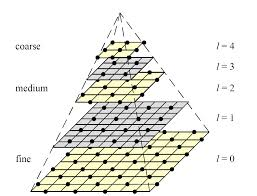
\includegraphics[width=.8\textwidth]{multilevel.png}
\caption{A MultiGrid hierarchy.\label{hierarchy}}
\end{center}
\end{figure}


Relaxation consists in the application of an iterative method, such as
Jacobi or Gauss-Seidel, to reduce highly oscillatory error components,
while the coarse-grid correction corresponds to the solution of the
resulting residual equation in an appropriately chosen coarse space
aimed at reducing the leftover error components. In the classical
multigrid approach, the coarser grid and the interpolation operator
for transfer the coarse-grid solution to the original (fine) grid are
predefined by the geometry of the problem. On the contrary, AMG
methods address this setup phase, known as \emph{coarsening process},
in an automatic way without using any explicit knowledge of the given
problem and relying only on system matrix entries. In this work we
refer to an algebraic coarsening process based on aggregation of
unknowns, where coarse-grid unknowns are agglomerates of the original
unknowns. In particular, AMG preconditioners available in MLD2P4 rely
on a decoupled version of \emph{the smoothed aggregation} algorithm
described in~\cite{BrezinaVanek96,BrezinaVanek99}. This procedure is
currently implemented on the host CPUs, therefore, for sake of space,
we refer the reader to~\cite{mld2p4-2-guide} for more details on the
algorithm and its parallel implementation. 
Our main aim here is to describe all the main Linear Algebra
operations needed for the application of the AMG preconditioner within
an iterative  linear solver, since their efficient implementation on
GPUs was the main focus of this work. 

The application phase of an AMG preconditioner is also known as
multi-grid cycle, the most widely used is the so called symmetric
V-cycle, described in Fig.~\ref{Vcycle}, where an AMG hierarchy of
$nlev$ prolongator operators $P^k$ and of corresponding coarse
matrices obtained by the standard variational approach
$A^{k+1}=(P^{k+1})^TA^kP^{k+1}$ have been built in the setup
phase. \textbf{Immagino che la formulazione del sistema lineare Ax=b
  (con A spd) sia stata definita prima da qualche parte}. 
\begin{figure}[t]
\begin{center}
\framebox{
\begin{minipage}{.85\textwidth}
\begin{tabbing}
\quad \=\quad \=\quad \=\quad \\[-3mm]
procedure V-cycle$\left(k,A^k,b^k,x^k\right)$ \\[2mm]
\>if $\left(k \ne nlev \right)$ then \\[1mm]
\>\> $x^k = x^k + (M^k)^{-1} \left(b^k - A^k x^k\right)$ \\[1mm]
\>\> $b^{k+1} = (P^{k+1})^T\left(b^k - A^k x^k\right)$ \\[1mm]
\>\> $x^{k+1} =$ V-cycle$\left(k+1,A^{k+1},b^{k+1},0\right)$ \\[1mm]
\>\> $x^k = x^k + P^{k+1} x^{k+1}$ \\[1mm]
\>\> $x^k = x^k + ((M^k)^T)^{-1} \left(b^k - A^k x^k\right)$ \\[1mm]
\>else \\[1mm]
\>\> $x^k = \left(A^k\right)^{-1} b^k$\\[1mm]
\>endif \\[1mm]
\>return $x^k$ \\[1mm]
end
\end{tabbing}
\end{minipage}
}
\caption{V-cycle preconditioner.\label{Vcycle}}
\end{center}
\end{figure}

We observe that in Fig.~\ref{Vcycle}, $M^k$ represents the matrix
operator corresponding to the basic iterative method applied at the
level $k$ for relaxation. 
Main computational kernels in the application of the preconditioner
are then sparse matrix-vector multiplications and inversion of the
matrix operator $M^k$. In the simple case of Jacobi method,
$M^k=diag(A^k)$, therefore it corresponds to a highly parallel vector
update operation. On the other hand, more robust iterative methods,
such as the Gauss-Seidel method or incomplete factorizations, are
often required for improving convergence rate of the preconditioner in
the solution of general linear systems. In that cases the inversion of
the corresponding matrix operators require the solution of triangular
systems that is an intrinsically sequential kernel. Therefore, an
efficient parallel implementation of the V-cycle application is
strictly related to an efficient implementation of the sparse
matrix-vector multiplication and to the availability of iterative
methods which can be formulated in terms of that kernel and possible
vector updates. 
\textbf{Immagino che l'utilita' di una fase di applicazione
  particolarmente efficiente, causa necessita' frequente di
  applicazione in metodi non lineari e/o risoluzione di sistemi
  multipli sia stata evidenziata nell'in troduzione}.
